\def\year{2019}\relax
\documentclass[letterpaper]{article} % DO NOT CHANGE THIS
\usepackage{aaai19}  % DO NOT CHANGE THIS
\usepackage{times}  % DO NOT CHANGE THIS
\usepackage{helvet} % DO NOT CHANGE THIS
\usepackage{courier}  % DO NOT CHANGE THIS
\usepackage[hyphens]{url}  % DO NOT CHANGE THIS
\usepackage{graphicx} % DO NOT CHANGE THIS
\urlstyle{rm} % DO NOT CHANGE THIS
\def\UrlFont{\rm}  % DO NOT CHANGE THIS
\usepackage{graphicx}  % DO NOT CHANGE THIS
\frenchspacing  % DO NOT CHANGE THIS
\setlength{\pdfpagewidth}{8.5in}  % DO NOT CHANGE THIS
\setlength{\pdfpageheight}{11in}  % DO NOT CHANGE THIS
\usepackage{amsmath, amssymb}
\graphicspath{{images/}}
\nocopyright
\usepackage{array}
\usepackage{caption,subcaption}
\usepackage{xcolor}
\usepackage[outputdir=output]{minted}
\usepackage{changepage}
%PDF Info Is REQUIRED.
% For /Author, add all authors within the parentheses, separated by commas. No accents or commands.
% For /Title, add Title in Mixed Case. No accents or commands. Retain the parentheses.
\pdfinfo{
/Title (Neural Networks)
/Author (Mark Wesley Harris)
} %Leave this	
% /Title ()
% Put your actual complete title (no codes, scripts, shortcuts, or LaTeX commands) within the parentheses in mixed case
% Leave the space between \Title and the beginning parenthesis alone
% /Author ()
% Put your actual complete list of authors (no codes, scripts, shortcuts, or LaTeX commands) within the parentheses in mixed case. 
% Each author should be only by a comma. If the name contains accents, remove them. If there are any LaTeX commands, 
% remove them. 

% DISALLOWED PACKAGES
% \usepackage{authblk} -- This package is specifically forbidden
% \usepackage{balance} -- This package is specifically forbidden
% \usepackage{caption} -- This package is specifically forbidden
% \usepackage{color (if used in text)
% \usepackage{CJK} -- This package is specifically forbidden
% \usepackage{float} -- This package is specifically forbidden
% \usepackage{flushend} -- This package is specifically forbidden
% \usepackage{fontenc} -- This package is specifically forbidden
% \usepackage{fullpage} -- This package is specifically forbidden
% \usepackage{geometry} -- This package is specifically forbidden
% \usepackage{grffile} -- This package is specifically forbidden
% \usepackage{hyperref} -- This package is specifically forbidden
% \usepackage{navigator} -- This package is specifically forbidden
% (or any other package that embeds links such as navigator or hyperref)
% \indentfirst} -- This package is specifically forbidden
% \layout} -- This package is specifically forbidden
% \multicol} -- This package is specifically forbidden
% \nameref} -- This package is specifically forbidden
% \natbib} -- This package is specifically forbidden -- use the following workaround:
% \usepackage{savetrees} -- This package is specifically forbidden
% \usepackage{setspace} -- This package is specifically forbidden
% \usepackage{stfloats} -- This package is specifically forbidden
% \usepackage{tabu} -- This package is specifically forbidden
% \usepackage{titlesec} -- This package is specifically forbidden
% \usepackage{tocbibind} -- This package is specifically forbidden
% \usepackage{ulem} -- This package is specifically forbidden
% \usepackage{wrapfig} -- This package is specifically forbidden
% DISALLOWED COMMANDS
% \nocopyright -- Your paper will not be published if you use this command
% \addtolength -- This command may not be used
% \balance -- This command may not be used
% \baselinestretch -- Your paper will not be published if you use this command
% \clearpage -- No page breaks of any kind may be used for the final version of your paper
% \columnsep -- This command may not be used
% \newpage -- No page breaks of any kind may be used for the final version of your paper
% \pagebreak -- No page breaks of any kind may be used for the final version of your paperr
% \pagestyle -- This command may not be used
% \tiny -- This is not an acceptable font size.
% \vspace{- -- No negative value may be used in proximity of a caption, figure, table, section, subsection, subsubsection, or reference
% \vskip{- -- No negative value may be used to alter spacing above or below a caption, figure, table, section, subsection, subsubsection, or reference

\setcounter{secnumdepth}{0} %May be changed to 1 or 2 if section numbers are desired.

% The file aaai19.sty is the style file for AAAI Press 
% proceedings, working notes, and technical reports.
%
\setlength\titlebox{2.5in} % If your paper contains an overfull \vbox too high warning at the beginning of the document, use this
% command to correct it. You may not alter the value below 2.5 in
\title{Neural Networks}
%Your title must be in mixed case, not sentence case. 
% That means all verbs (including short verbs like be, is, using,and go), 
% nouns, adverbs, adjectives should be capitalized, including both words in hyphenated terms, while
% articles, conjunctions, and prepositions are lower case unless they
% directly follow a colon or long dash
\author{Mark Wesley Harris\\ % All authors must be in the same font size and format. Use \Large and \textbf to achieve this result when breaking a line
% If you have multiple authors and multiple affiliations
% use superscripts in text and roman font to identify them. For example, Sunil Issar,\textsuperscript{\rm 2} J. Scott Penberthy\textsuperscript{\rm 3} George Ferguson,\textsuperscript{\rm 4} Hans Guesgen\textsuperscript{\rm 5}. Note that the comma should be placed BEFORE the superscript for optimum readability
University of Colorado Colorado Springs\\
wharris2@uccs.edu % email address must be in roman text type, not monospace or sans serif
}
\begin{document}

\maketitle

\begin{abstract}
Neural Networks are a widely studied topic in machine learning.
Through our experiments, we demonstrate the power of
Artifical Neural Networks and Convolutional Neural Networks
to learn complex data patterns and make better predictions on test data.
We show that CNN's are particularly suited for advanced image processing,
and explore the importance of hyperparameters for networks in general.
\end{abstract}

\section{Introduction}
Machine Learning is a powerful tool for extracting information from sets of data.
As we discovered previously, different types of classification methods can be used to
train algorithms to learn trends in data.
The ultimate goal of a classifier is to make predictions on new information;
however, many machine learning methods are not suitable for
complex problems, such as machine vision or natural language processing.
The demand for better classification models led to the development of Neural Networks,
which provided the foundations of powerful machine learning algorithms.
Tougher problems are being solved every day, by applying innovations and creating new types of networks.

Here we study how these networks behave and also observe the benefits of convolution,
pooling, and dropout.
We implement a simple ANN from scratch, as well as two CNN implementations written in
Python and R.
The performance of each model is evaluated using 3 popular image datasets, MNIST, CIFAR-10, and CIFAR-100.
The basic models constructed here are not suited for surpassing real benchmarks,
however they serve to illustrate the power and applications of Neural Networks in general.

\section{Neural Networks}
The discoveries from Logistic Regression were made more powerful through the invention of Artificial Neural Networks (ANN's).
ANN's simulate the interactions of neurons to obtain weights that can be used
for making predictions on more complex problems.
Each neuron makes use of the sigmoid function explored in Logistic Regression, to help extract features
as information is processed. Nodes closer to the input layer are used to extract simple features,
while those further down have the ability to find more complex ones.
Researchers have studied the implications of ANN's,
and were able to show that ANN's of a single hidden layer with non-polynomial activation function are
universal predictors \cite{universal}. In practice, however, many more layers and complexities are added to
speed up processing and give better results than training a single layer network.

\subsection{Forward and Backward Propagation}
A basic dense ANN is comprised of one input layer, one hidden layer,
and one output layer, each of variable sizes.
Let these sizes be called $N^{(i)}$, $N^{(h)}$, and $N^{(o)}$, respectively.
The forward and backward propagation
is calculated intrinsically using matrix representations of the
weights ($\mathbf{w_1},\mathbf{w_2}$) and biases ($\mathbf{b_0},\mathbf{b_1}$).
The sizes of matrices $\mathbf{w}$ and $\mathbf{b}$ are dependent upon where they are used
in the network.
Since $\mathbf{w_1}$ and $\mathbf{b_1}$ are used in the single hidden layer,
they have shapes
($N^{(h)}, N^{(i)}$) and ($N^{(h)}, 1$).
Similarly, $\mathbf{w_2}$ and $\mathbf{b_2}$ have shapes
($N^{(o)}, N^{(h)}$) and ($N^{(o)}, 1$).

\begin{equation}
\label{eq:forward}
\hat{\mathbf{y}} = \sigma(\mathbf{w}^T\mathbf{x} + \mathbf{b}) \text{, where } \sigma(\mathbf{x}) = \frac{1}{1 + e^{-\mathbf{x}}}
\end{equation}

Forward propagation is defined in Equation \ref{eq:forward}.
Notice that the activation function is denoted as $\sigma$.
Given a multi-class classification problem,
the definition of $\sigma$ actually changes to softmax for the final output layer.
Thus the activation function of the last layer is represented as
$\sigma = \frac{e^{x_i}}{\sum_{i=0}^{i=n}e^{x_i}}$,
where $n$ is the number of unique classes.

Backward propagation involved more calculations using $\mathbf{w}$ and $\mathbf{b}$.
Essentially, we are solving for the following value.

\begin{equation}
\label{eq:backward}
\begin{split}
\frac{\partial \mathcal{L}}{\partial w_j} &=
\frac{\partial \mathcal{L}}{\partial o_j}
\frac{\partial o_j}{\partial \text{net}_j}
\frac{\partial \text{net}_j}{\partial w_j} \\
&=
\frac{\hat{\mathbf{y}} - \mathbf{y}}{\hat{\mathbf{y}}(1 - \hat{\mathbf{y}})}
[\hat{\mathbf{y}}(1 - \hat{\mathbf{y}})]
w_j \\
&=
(\hat{\mathbf{y}} - \mathbf{y})w_j
\end{split}
\end{equation}

The same calculation is performed for the biases, $\mathbf{b}$.
After further simplification, we obtain the following equations.
Note that in either partial derivation of $\mathcal{L}$,
$m$ represents the number of example vectors.

\begin{equation}
\frac{\partial \mathcal{L}}{\partial \mathbf{w}} =
\frac{\mathbf{w}(\hat{\mathbf{y}} - \mathbf{y})^T}{m}
\end{equation}
\begin{equation}
\frac{\partial \mathcal{L}}{\partial \mathbf{b}} =
\frac{\sum_{i=1}^{m}(\hat{y}^{(i)} - y^{(i)})}{m}
\end{equation}

\subsection{Convolutional Neural Networks}
there are some situations where a basic ANN is impractical.
Researchers found that more abstract learning goals, such as edge detection,
were difficult to implement in a basic network.
In fact, appropriate solutions for computer vision and image processing problems were still unobtainable
with the ANN architectures discussed above.
In an effort to help with learning these types of features, the idea of convolution was applied
to create a new class of Neural Networks, called
Convolutional Neural Networks (CNN's).

The general concept of convolution is shown in Figure \ref{fig:convolution}.
Convolution involves processing a small section of an image, in order to obtain a new representation called a ``filter''
\cite{imagenet}.
The filter allows for extracting high-level features more easily,
and it has been found that it also helps keep the relationship of pixels to their neighbors
which would otherwise be overlooked by an ANN.

\begin{figure}[htbp]
\centerline{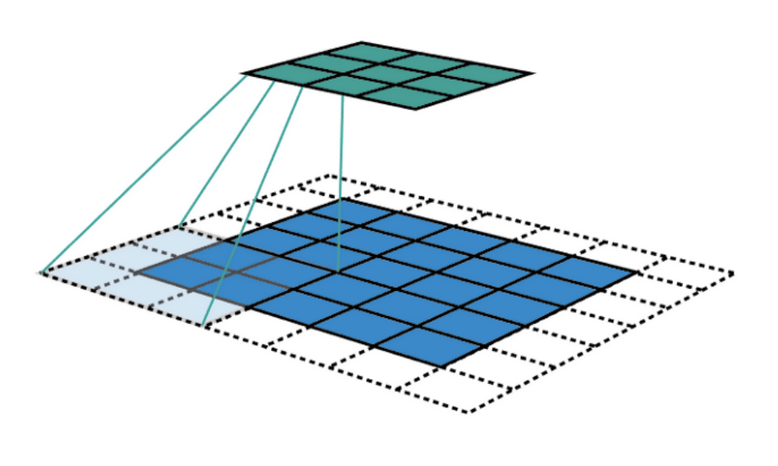
\includegraphics[width=6cm]{convolution.png}}
\caption{An example of convolution, where a portion of the input data is selected and processed.}
\label{fig:convolution}
\end{figure}

Convolution is only one of the many advancements commonly used in CNN's --
another is called pooling, where data is compressed to amplify extractable features.
Figure \ref{fig:max_pooling} shows an example of max pooling, which is popular in image processing.
Our implementation used a combination of convolution, max pooling, and dropout layers
for training the CNN's we evaluated.
There are other possible applications of these and other network layers,
however they are not explored here.

\begin{figure}[htbp]
\centerline{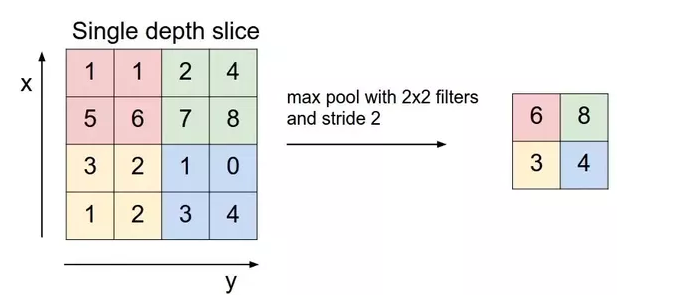
\includegraphics[width=7cm]{max_pooling.png}}
\caption{Max pooling with 2 x 2 filters and stride 2.}
\label{fig:max_pooling}
\end{figure}

\section{Implementation}
The Keras API was used for both the Python and R library implementations.
The Python program obtained Keras via the TensorFlow API \cite{python}.
The R script was based off of an R Studio Blog post,
which gave enough information to build the CNN models \cite{r}.
The Keras library provided appropriate means of evaluation,
while analysis of our implementation was aided by observing confusion matrices
and losses on test data.

\subsection{Evaluation}
There are ample datasets to choose from to evaluate our network implementations.
We used the MNIST, CIFAR-10, and CIFAR-100 datasets --
The MNIST dataset is made up of 60,000 (28 x 28) pixel images with only one channel (grey values),
while the CIFAR datasets contain 60,000 (32 x 32) with 3 channels (red, green,
and blue values).
Figure \ref{fig:datasets} shows random samples of 4 classes from each dataset.
Notice that MNIST is a dataset of handwritten digits, so in total it has 10 classes.
CIFAR-10 has 10 different classes of images, and CIFAR-100 has 100 different classes.
Each convolution layer for the library implementations uses 64 (3 x 3) filters with a stride of 1.
This results in a total of 64 (32 x 32 x 3) volumes for the CIFAR datasets,
and 64 (28 x 28 x 1) volumes for MNIST.

\begin{figure}[htbp]
\centering
\begin{subfigure}{0.115\textwidth}
  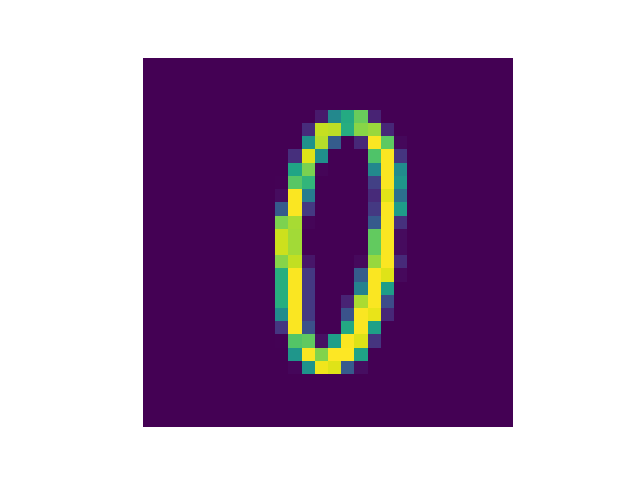
\includegraphics[width=\linewidth]{mnist_0.png}
  \caption{0}
\end{subfigure}\hfil
\begin{subfigure}{0.115\textwidth}
  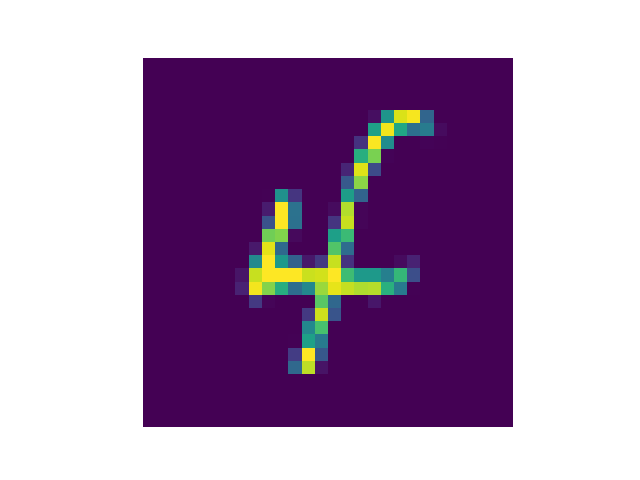
\includegraphics[width=\linewidth]{mnist_4.png}
  \caption{4}
\end{subfigure}\hfil
\begin{subfigure}{0.115\textwidth}
  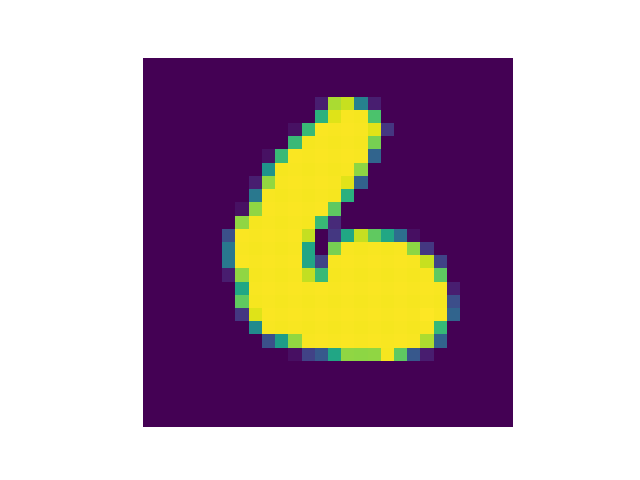
\includegraphics[width=\linewidth]{mnist_6.png}
  \caption{6}
\end{subfigure}\hfil
\begin{subfigure}{0.115\textwidth}
  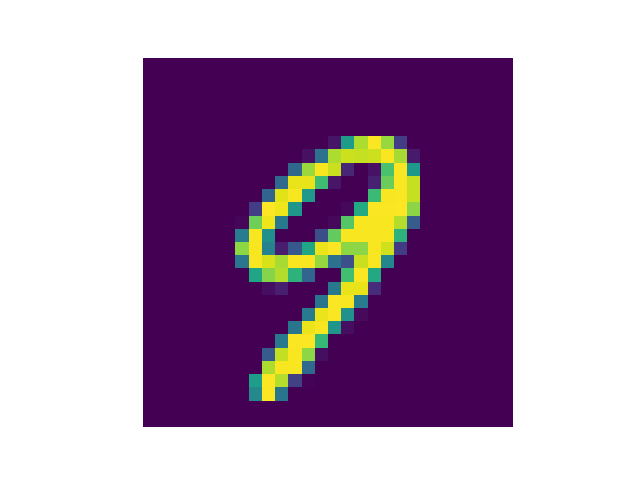
\includegraphics[width=\linewidth]{mnist_9.png}
  \caption{9}
\end{subfigure}
\begin{subfigure}{0.115\textwidth}
  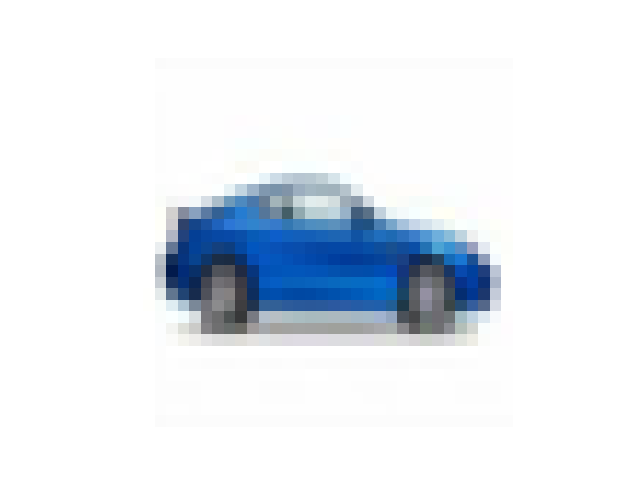
\includegraphics[width=\linewidth]{cifar-10_1.png}
  \caption{Automobile}
\end{subfigure}\hfil
\begin{subfigure}{0.115\textwidth}
  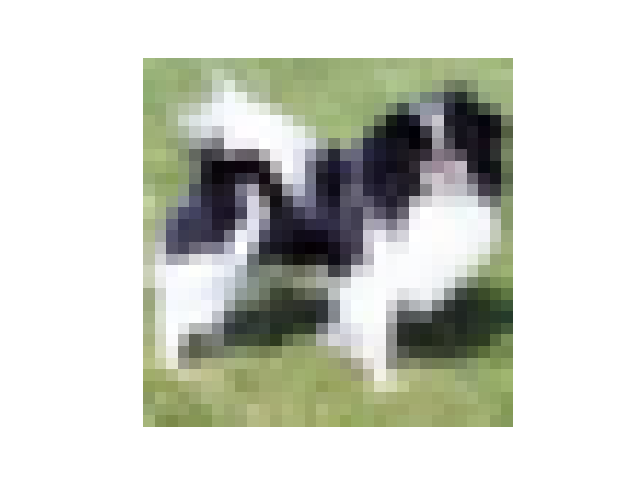
\includegraphics[width=\linewidth]{cifar-10_5.png}
  \caption{Dog}
\end{subfigure}\hfil
\begin{subfigure}{0.115\textwidth}
  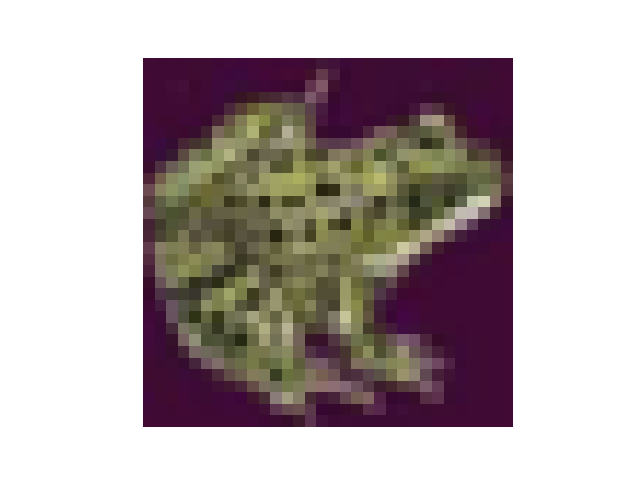
\includegraphics[width=\linewidth]{cifar-10_6.png}
  \caption{Frog}
\end{subfigure}\hfil
\begin{subfigure}{0.115\textwidth}
  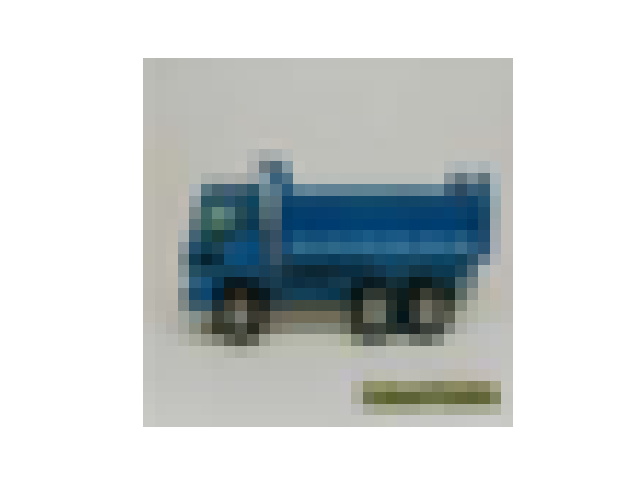
\includegraphics[width=\linewidth]{cifar-10_9.png}
  \caption{Truck}
\end{subfigure}
\begin{subfigure}{0.115\textwidth}
  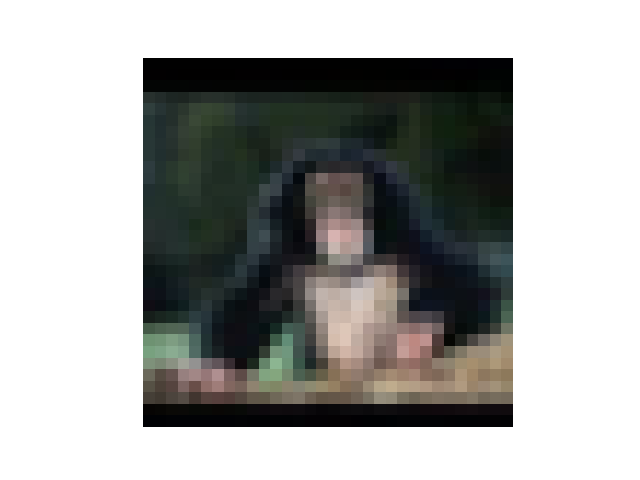
\includegraphics[width=\linewidth]{cifar-100_21.png}
  \caption{Chimpanzee}
\end{subfigure}\hfil
\begin{subfigure}{0.115\textwidth}
  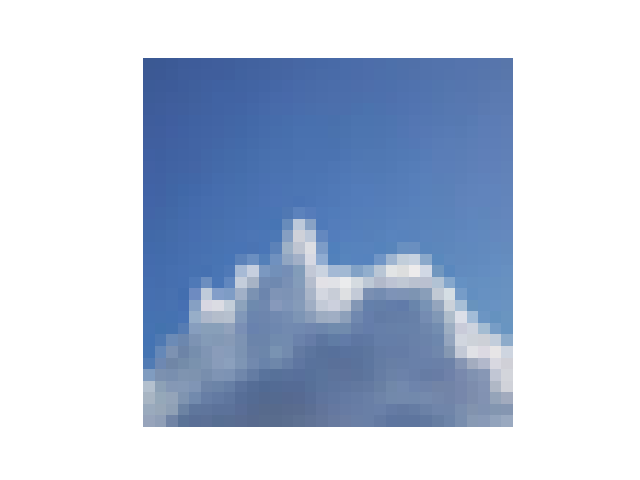
\includegraphics[width=\linewidth]{cifar-100_23.png}
  \caption{Cloud}
\end{subfigure}\hfil
\begin{subfigure}{0.115\textwidth}
  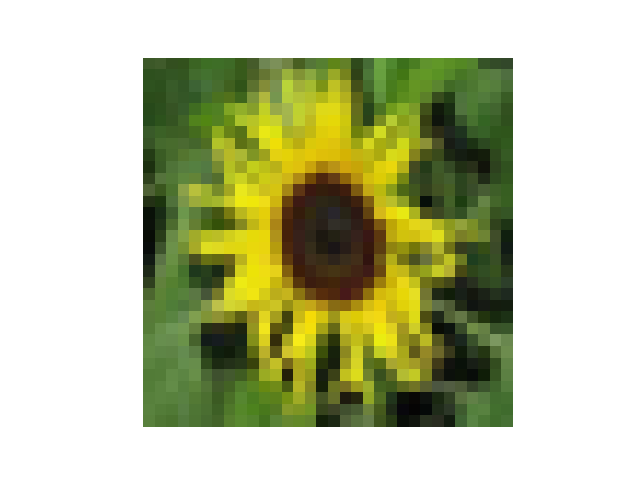
\includegraphics[width=\linewidth]{cifar-100_82.png}
  \caption{Sunflower}
\end{subfigure}\hfil
\begin{subfigure}{0.115\textwidth}
  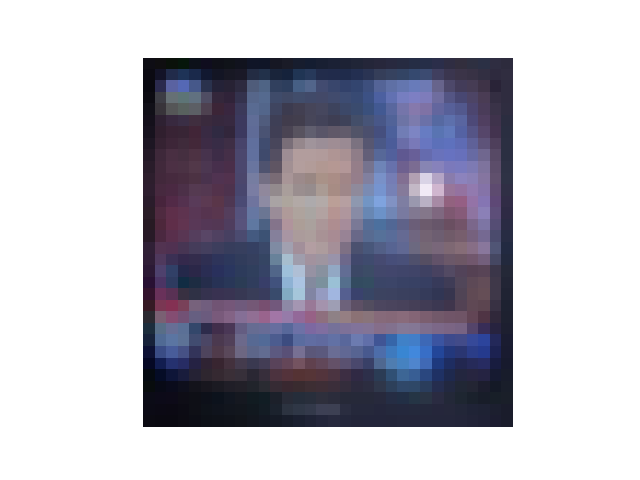
\includegraphics[width=\linewidth]{cifar-100_87.png}
  \caption{Man}
\end{subfigure}
\caption{Examples from the MNIST (a - d), CIFAR-10 (e - h), and
CIFAR-100 (i - l) datasets.}
\label{fig:datasets}
\end{figure}

\subsection{Challenges}
The most challenging part of implementation was working with the multiple datasets across
two different languages. While the datasets themselves are standardized, the method to import
and ultimately use the data in a network is ambiguous.
The MNIST dataset was imported using the TensorFlow API, while
we decided to import the CIFAR data from downloaded files.
The latter was very involved, especially for reshaping the channels of data for processing
by the network. We later discovered that while the TensorFlow API does not provide
a simple importer for the CIFAR datasets, the Keras API does.
Thus, the code we wrote for importing CIFAR could be replaced with a much simpler implementation.

Another challenge we faced was in training all 9 networks. It was found that for best results,
each network should be trained separately (or alternatively on different machines
with similar specs).
The number of epochs was kept to a minimum in order to have enough time for training and
evaluation of all networks, which is why further experimentation is needed for
truly determining the correct hyperparameters in each situation.

\section{Results}
\begin{table}[t]
\begin{centering}
\bgroup
\def\arraystretch{1.5}
\begin{tabular}{| m{0.17\textwidth} | m{0.0625\textwidth} | m{0.0625\textwidth} | m{0.0625\textwidth} |} 
\hline
Method & MNIST & CIFAR-10 & CIFAR-100 \\ 
\hline
\hline
Our Python NN & 0.56014 & 2.24362 & 4.61970 \\
\hline
\hline
Library Python CNN & 0.07083 & 1.36986 & 3.58488\\
\hline
Library R CNN & 0.03113 & 1.04461 & 2.81414 \\
\hline
\end{tabular}
\caption{Best losses found for each dataset evaluated with each model.}
\label{tbl:fits}
\egroup
\end{centering}
\end{table}

The results of our implementation for both of the CIFAR datasets was extremely poor
compared to our results on the MNIST dataset.
Even when the hyperparameters were tuned to achieve better results in the given
constraints,
it seems the basic ANN could not handle the increase in information by colored image data.
In an attempt to improve accuracy, CIFAR data was pooled from a 3,072 long vector down
to a length of 1,024.
We found this change did not affect results in a major way,
since ultimately the features were just as hard to extract.

Upon further examination of the confusion matrices, we determined the main cause of the
drop in performance for CIFAR datasets to stem from overfitting of the data.
The network was found to learn the weights and biases, however one or two examples were favored over the others.
This effect was compounded in the CIFAR-100 dataset, to the extent that the network at times learned to predict
only one of the 100 possible image classes.
This is the worst accuracy possible for the given problem.

The library implementations performed much better overall.
Table \ref{tbl:accuracies} shows how the number of convolution layers affects network performance,
in this case a comparison of 2 to 6 layers.
While the number of convolution layers affected results very little for the R library implementation,
the Python model suffered greatly with the increase in convolutions. By studying the loss over the course of
training, we identified a clear point during training where accuracy plummeted.
The end result was a highly over-fit model.
%This behavior offers us insight into why our implementations
%for MNIST worked comparably well to the library results, while the CIFAR datasets showed the same
%trend of over-fitting.
More examination for the implementation would be necessary to fix this problem.
The minimal effects for R script was likely due to the high number of filters used for each layer.
A useful future experiment would be to examine the effect the number of filters has the network in each case,
as well as how varying training epochs and hidden layers could improve results.

\begin{table}[t]
\begin{centering}
\bgroup
\def\arraystretch{1.5}
\begin{tabular}{| m{0.17\textwidth} | m{0.0625\textwidth} | m{0.0625\textwidth} | m{0.0625\textwidth} |} 
\hline
Method & MNIST & CIFAR-10 & CIFAR-100 \\ 
\hline
\hline
\multicolumn{4}{|c|}{Python} \\
\hline
2 Convolution Layers & 0.9838 & 0.6459 & 0.3002 \\
\hline
6 Convolution Layers & 0.0895 & 0.0998 & 0.0099 \\
\hline
\multicolumn{4}{|c|}{R} \\
\hline
2 Convolution Layers & 0.9916 & 0.685 & 0.344 \\
\hline
6 Convolution Layers & 0.9905 & 0.688 & 0.343 \\
\hline
\end{tabular}
\caption{Average accuracies found for each dataset given different model architectures.}
\label{tbl:accuracies}
\egroup
\end{centering}
\end{table}

Figure \ref{fig:losses} shows how losses varied over the course of training our non-library implementations.
Each subplot reflects 4 different distributions collected for different combinations of hyperparameters over each dataset.
In general, the learning parameter $\lambda$ and number of hidden layer nodes were permuted with
low and high values. The number of training epochs was kept the same, in order to give a standard basis of comparison
between datasets. However, it is worth noting that training on the CIFAR datasets benefited from a higher number of
epochs. In general, the CIFAR data gave better output for higher-precision hyperparameters. This is why $\lambda$
was decreased and the number of hidden layer nodes was increased for evaluations,
compared to the values used for training on the MNIST dataset.
The best hyperparameters found for each dataset are enumerated in Table \ref{tbl:params}.

\begin{figure}[htbp]
\centerline{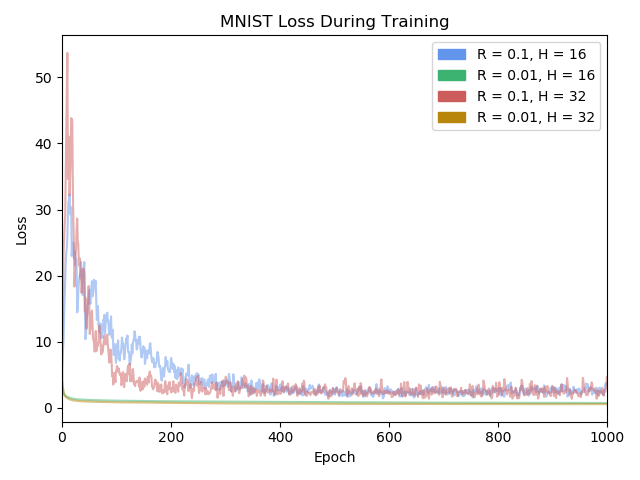
\includegraphics[width=9cm]{mnist_loss.png}}
\centerline{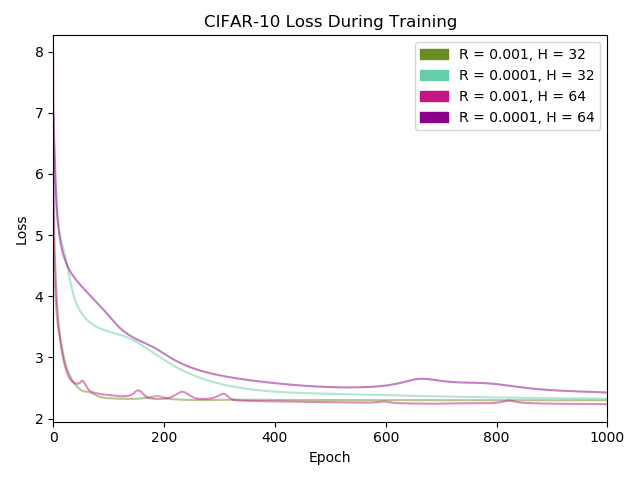
\includegraphics[width=9cm]{cifar-10_loss.png}}
\centerline{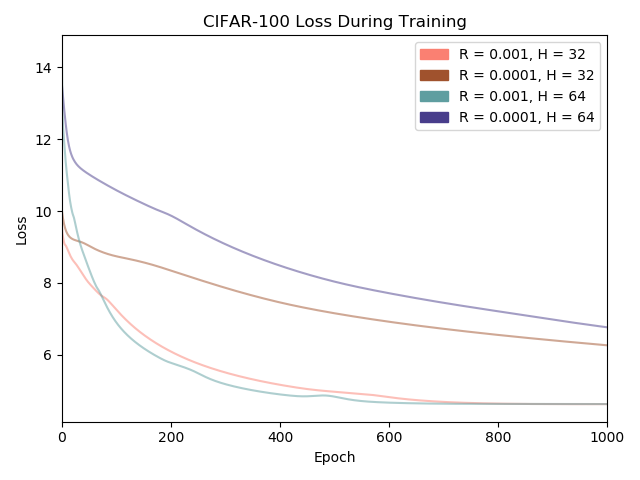
\includegraphics[width=9cm]{cifar-100_loss.png}}
\caption{Losses for our implementation during training on each dataset with different hyperparameters.}
\label{fig:losses}
\end{figure}

\begin{table}[t]
\begin{centering}
\bgroup
\def\arraystretch{1.5}
\begin{tabular}{| m{0.17\textwidth} | m{0.0625\textwidth} | m{0.0625\textwidth} | m{0.0625\textwidth} |} 
\hline
Parameter & MNIST & CIFAR-10 & CIFAR-100 \\ 
\hline
\hline
Learning Parameter & 0.01 & 0.001 & 0.001 \\
\hline
Hidden Nodes & 32 & 32 & 64 \\
\hline
\end{tabular}
\caption{The best hyperparameters found out of those experimented with.}
\label{tbl:params}
\egroup
\end{centering}
\end{table}

\section{Conclusion}
We successfully trained 3 networks over 3 different datasets
and were able to evaluate them with varying parameters.
Analyzing our results, it is clear that hyperparameters play a larger role in network performance
for ANN's and CNN's than they did with Logistic Regression and simpler machine learning models.
A major problem for running our implementation on the CIFAR datasets was overfitting
of the data during training.
Overfitting is not uncommon for neural networks, and is one of the reasons CNN's are used in place of ANN's for
processing image data \cite{imagenet}.
If nothing else, the polarized results of our networks proved that
ANN's are suboptimal for situations where the data is more complex,
or has complex spatial relationships with surrounding data.
The use of convolutions not only made processing data faster,
but also increased the prediction power of the trained network.
While the complexity of a network itself can have unexpected consequences on training,
our results of comparing ANN's and CNN's show
there is a clear benefit to processing data in smart ways.
Using the right network for a given problem can
improve feature extraction and ultimately the resulting predictions on test data.

\bibliography{report}
\bibliographystyle{aaai}

\onecolumn

\pagebreak

\begin{center}
\section*{Appendix}
\label{app:b}
\end{center}

\bigskip

\footnotesize{
\begin{minted}{python}
# nn.py
import matplotlib.pyplot as plt
import numpy as np
from sklearn.metrics import classification_report, confusion_matrix
import utils as utils

########################
#  NETWORK DEFINITION  #
########################

# Define sigmoid function as activation.
def activation(x):
    return 1 / (1 + np.exp(-x))

# Define softmax function as final layer activation.
def final(x):
    return np.exp(x) / np.sum(np.exp(x), axis=0)

# Define initialization step.
def initialize_parameters(shape):
    # Initialize weights for input and hidden layer.
    w = [np.random.randn(shape[1], shape[0]),  # (hidden, input )
         np.random.randn(shape[2], shape[1])]  # (output, hidden)

    # Initialize biases for input and hidden layer.
    b = [np.zeros((shape[1], 1)),              # (hidden, 1     )
         np.zeros((shape[2], 1))]              # (output, 1     )

    # Return the weights and biases.
    return w, b

# Define forward step, return outputs of each layer.
def forward_step(x, w, b):
    res = []
    res.append(activation(np.matmul(w[0], x) + b[0]))
    res.append(final(np.matmul(w[1], res[0]) + b[1]))

    return res

# Define backward step, return calculated gradients.
def backward_step(x, y, outs, w):
    # Initialize result and helper variables.
    res = []
    d2 = outs[1] - y
    d1 = np.multiply(np.dot(w[1].T, d2), 1 - np.power(outs[0], 2))

    res.append([np.dot(d1, x.T) / float(len(x)),
                np.sum(d1, axis=1, keepdims=True) / float(len(x))])

    res.append([np.dot(d2, outs[0].T) / float(len(x)),
                np.sum(d2, axis=1, keepdims=True) / float(len(x))])

    return res

# Define update step.
def gradient_descent(w, b, grads, alpha):
    # Update weights.
    for i, w_i in enumerate(w):
        w[i] = w_i - alpha * grads[i][0]

    # Update biases.
    for i, b_i in enumerate(b):
        b[i] = b_i - alpha * grads[i][1]

    return w, b

########################
#  NETWORK EVALUATION  #
########################

# Define loss calculation for Gradient Descent.
def loss(y_real, y_pred):
    return -np.sum(np.multiply(y_real, np.log(y_pred))) / float(y_real.shape[1])

# Define accuracy calculation.
def accuracy(y_real, y_pred):
    s = 0
    for i in range(len(y_real)):
        if y_real[i] == y_pred[i]:
            s += 1

    return s / float(len(y_real))

# Define confusion matrix calculation.
def confusion(y_real, y_pred):
    predictions = np.argmax(y_pred, axis=0)
    labels = np.argmax(y_real, axis=0)

    print(confusion_matrix(predictions, labels))
    print(classification_report(predictions, labels))

########################
########  MAIN  ########
########################

# Define how to run the dense Neural Network.
def neural_network(dataset, num_epochs, net_hid, alpha):
    x_train, y_train, x_test, y_test = [], [], [], []
    net_inp, net_out = 1, 1
    losses = []

    if dataset == 'MNIST':
        # Import training and testing data from TensorFlow API.
        x_train, y_train, x_test, y_test = utils.import_MNIST()
        print(x_train.shape, y_train.shape)
        net_inp = x_train.shape[0]
        net_out = 10
    elif dataset == 'CIFAR-10':
        # Import training and testing data from files.
        x_train, y_train, x_test, y_test = utils.import_CIFAR(10)
        print(x_train.shape, y_train.shape)
        net_inp = x_train.shape[0]
        net_out = 10
    elif dataset == 'CIFAR-100':
        # Import training and testing data from files.
        x_train, y_train, x_test, y_test = utils.import_CIFAR(100)
        print(x_train.shape, y_train.shape)
        net_inp = x_train.shape[0]
        net_out = 100
    else:
        print('Please enter a valid dataset [MNIST, CIFAR-10, CIFAR-100]')
        return

    net_shape = (net_inp, net_hid, net_out)

    # Initialize network weights and biases.
    w, b = initialize_parameters(net_shape)

    for i in range(num_epochs):
        res = forward_step(x_train, w, b)

        grads = backward_step(x_train, y_train, res, w)
        w, b = gradient_descent(w, b, grads, alpha)

        losses.append(loss(y_train, res[1]))
        if (i % 100 == 0):
            print('{0}: {1}'.format(i, losses[i]))

    # Create final outputs.
    res = forward_step(x_test, w, b)
    confusion(y_test, res[1])

    return losses
\end{minted}

\bigskip

\begin{minted}{python}
# utils.py
from collections import defaultdict
import copy as copy
from keras.utils import to_categorical
import matplotlib.pyplot as plt
import matplotlib.patches as mpatches
import numpy as np
import os as os
import pickle as pickle
import tensorflow as tf
import tensorflow_datasets as tfds

# Make a directory if it doesn't exist.
def make_dir(path):
    if not os.path.exists(path):
        os.mkdir(path)

# Encode data into categories.
def encode(data):
    return np.array(to_categorical(data))

# Decode data from categories.
def decode(data):
    return np.argmax(data)

# Shuffle two arrays in the same way.
def shuffle_data(x, y):
    for i in reversed(range(1, len(x))):
        # pick an element in x[:i] with which to exchange x[i]
        j = np.random.randint(0, i)
        x_i = np.array(x[i])
        x_j = np.array(x[j])
        x[i], x[j] = x_j, x_i
        y_i = np.array(y[i])
        y_j = np.array(y[j])
        y[i], y[j] = y_j, y_i

    return x, y

# Save test image to check import.
def test_import(data, path):
    fig = plt.figure()
    plt.axis("off")
    plt.imshow(data)
    fig.savefig(path)
    plt.clf()
    print('Saved image to: ' + path)

# Import MNIST training and testing data from TensorFlow API.
def import_MNIST():
    print('Loading MNIST Dataset...')
    (x_train_d, y_train), (x_test_d, y_test) = tf.keras.datasets.mnist.load_data()

    x_train = []
    shape = x_train_d.shape
    for i in range(shape[0]):
        x_train.append(x_train_d[i].reshape(shape[1] * shape[2]) / 255.0)
    x_train, y_train = shuffle_data(x_train, y_train)

    x_test = []
    shape = x_test_d.shape
    for i in range(shape[0]):
        x_test.append(x_test_d[i].reshape(shape[1] * shape[2]) / 255.0)
    x_test, y_test = shuffle_data(x_test, y_test)

    # Save test import.
    path = 'mnist/'
    make_dir(path)
    test_import(x_train[0].reshape(28, 28), path + str(y_train[0]) + '.png')

    return np.array(x_train).T, encode(y_train).T, np.array(x_test).T, encode(y_test).T

# Import CIFAR training and testing data from stored files.
def import_CIFAR(cifar_type):
    if cifar_type == 10:
        path = 'cifar-10'
    else:
        path = 'cifar-100'

    x_train, y_train, x_test, y_test, meta = helper_CIFAR(path)
    x_train, y_train = shuffle_data(x_train, y_train)
    x_test, y_test = shuffle_data(x_test, y_test)

    return np.array(x_train).T, encode(y_train).T, np.array(x_test).T, encode(y_test).T

# Helper function for splitting CIFAR training and testing data.
def helper_CIFAR(cifar_type):
    prefix = '../../../source/'
    images = None
    labels = None

    if cifar_type == 'cifar-10':
        meta_postfix = '/batches.meta'
        with open('{0}{1}{2}'.format(prefix, cifar_type, meta_postfix), 'rb') as f:
            meta = pickle.load(f, encoding='bytes')

        data_postfix = '/data_batch_'
        for i in range(1, 6):
            path = '{0}{1}{2}{3}'.format(prefix, cifar_type, data_postfix, i)
            print('Loading path: ' + path)
            with open(path, 'rb') as f:
                pickle_dict = pickle.load(f, encoding='bytes')

            pickle_images = np.array(pickle_dict[b'data'], dtype=np.uint8)
            if images is not None:
                images = np.concatenate([images, pickle_images])
            else:
                images = pickle_images

            pickle_labels = np.array(pickle_dict[b'labels'], dtype=np.uint8)
            if labels is not None:
                labels = np.concatenate([labels, pickle_labels])
            else:
                labels = pickle_labels
        
        data_postfix = '/test_batch'
        path = '{0}{1}{2}'.format(prefix, cifar_type, data_postfix)
        print('Loading path: ' + path)
        with open(path, 'rb') as f:
            pickle_dict = pickle.load(f, encoding='bytes')

        pickle_images = np.array(pickle_dict[b'data'], dtype=np.uint8)
        if images is not None:
            images = np.concatenate([images, pickle_images])
        else:
            images = pickle_images

        pickle_labels = np.array(pickle_dict[b'labels'], dtype=np.uint8)
        if labels is not None:
            labels = np.concatenate([labels, pickle_labels])
        else:
            labels = pickle_labels
    else:
        meta_postfix = '/meta'
        with open('{0}{1}{2}'.format(prefix, cifar_type, meta_postfix), 'rb') as f:
            meta = pickle.load(f, encoding='bytes')

        data_postfix = '/train'
        path = '{0}{1}{2}'.format(prefix, cifar_type, data_postfix)
        print('Loading path: ' + path)
        with open(path, 'rb') as f:
            pickle_dict = pickle.load(f, encoding='bytes')

        for key, value in pickle_dict.items():
            print(key)

        pickle_images = np.array(pickle_dict[b'data'], dtype=np.uint8)
        if images is not None:
            images = np.concatenate([images, pickle_images])
        else:
            images = pickle_images

        pickle_labels = np.array(pickle_dict[b'fine_labels'], dtype=np.uint8)
        if labels is not None:
            labels = np.concatenate([labels, pickle_labels])
        else:
            labels = pickle_labels

        data_postfix = '/test'
        path = '{0}{1}{2}'.format(prefix, cifar_type, data_postfix)
        print('Loading path: ' + path)
        with open(path, 'rb') as f:
            pickle_dict = pickle.load(f, encoding='bytes')

        pickle_images = np.array(pickle_dict[b'data'], dtype=np.uint8)
        if images is not None:
            images = np.concatenate([images, pickle_images])
        else:
            images = pickle_images

        pickle_labels = np.array(pickle_dict[b'fine_labels'], dtype=np.uint8)
        if labels is not None:
            labels = np.concatenate([labels, pickle_labels])
        else:
            labels = pickle_labels

    # Save test import.
    path = cifar_type + '/'
    make_dir(path)
    index = np.random.randint(0, len(images))
    test_import(images[index].reshape(3, 32, 32).transpose(1,2,0),
                path + str(labels[index]) + '.png')

    # Reshape image data.
    pixel_data = []
    for i in range(len(images)):
        pixels = images[i].reshape(3, 32, 32).transpose(1, 2, 0)
        transformed = pixels.sum(axis=2)
        pixel_data.append(transformed.reshape(32 * 32))

    print(np.array(pixel_data).shape)

    # Split into training and testing data.
    split = 50000
    x_train, x_test = np.array(pixel_data)[:split], np.array(pixel_data)[split:]
    y_train, y_test = labels[:split], labels[split:]

    print('Metadata: ', meta)
    print('Images: ', images.shape)
    print('Labels: ', labels.shape)
    return x_train / (3 * 255.0), y_train, x_test / (3 * 255.0), y_test, meta

# Definition for plotting values.
def plot_together(values, colors, labels, title, path, fit_flag):
    samples = len(values[0])
    x_axis = np.linspace(0, samples, samples, endpoint=True)
    patches = []
    
    # Plot values and fits.
    for i in range(len(values)):
        avg = np.average(values[i])
        plt.plot(x_axis, values[i], color=colors[i], alpha=0.5)
        if fit_flag:
            plt.plot(np.unique(x), np.poly1d(np.polyfit(x, values[i], 1))(np.unique(x)),
                     color=colors[i], linestyle='--')
        patches.append(mpatches.Patch(color=colors[i]))
        print(title + '[' + str(i) + ']: ' + str(avg))
    
    # Finish plot.
    plt.legend(patches, labels, loc='upper right')
    plt.xlabel('Epoch')
    plt.ylabel('Loss')
    plt.title(title)
    axes = plt.gca()
    axes.set_xlim([0, samples])
    plt.tight_layout()
    
    if os.path.exists(path):
        os.remove(path)
    plt.savefig(path)
    plt.clf()
\end{minted}

\bigskip

\begin{minted}{python}
# mnist.py (cifar-10 and cifar-100 are very similar)
# Modeled off of "The Sequential model API" (Keras Documentation)
# Source: https://keras.io/models/sequential/
from keras.models import Sequential
from keras.layers import Dense, Conv2D, Dropout, Flatten, MaxPooling2D
import matplotlib.pyplot as plt
import tensorflow as tf
import utils as utils

# Import training and testing data from TensorFlow API.
print('Loading MNIST Dataset...')
(x_train, y_train), (x_test, y_test) = tf.keras.datasets.mnist.load_data()

# Normalization
shape = (28, 28, 1)
x_train = x_train.reshape(x_train.shape[0], shape[0], shape[1], shape[2]) / 255.0
x_test = x_test.reshape(x_test.shape[0], shape[0], shape[1], shape[2]) / 255.0

# Create a Sequential base model.
model = Sequential()

# Add each layer to the model and set the shape for the nodes accordingly.
model.add(Conv2D(64, kernel_size=(3,3), input_shape=shape))
model.add(MaxPooling2D(pool_size=(2, 2)))
model.add(Flatten())
model.add(Dense(128, activation=tf.nn.relu))
model.add(Dropout(0.2))
model.add(Dense(10, activation=tf.nn.softmax))

# Compile the model and fit it with the training data.
model.compile(optimizer='adam', 
              loss='sparse_categorical_crossentropy', 
              metrics=['accuracy'])
model.fit(x=x_train,y=y_train, epochs=10)

# Evaluate the model.
evaluation = model.evaluate(x_test, y_test)
print(evaluation)
\end{minted}

\bigskip

\begin{minted}{r}
# mnist.r (cifar-10 and cifar-100 are very similar)
# Modeled off of "Keras for R Studio"
# Source: https://blog.rstudio.com/2017/09/05/keras-for-r/

if(!require(keras)) {
  install.packages("keras")
  install_keras()
}
library("keras")
setwd("./mnist/")

# Load dataset.
data <- dataset_mnist()
x_train <- data$train$x
y_train <- data$train$y
x_test <- data$test$x
y_test <- data$test$y

# Reshape data.
dim(x_train) <- c(nrow(x_train), 28, 28, 1)
dim(x_test) <- c(nrow(x_test), 28, 28, 1)
x_train <- x_train / 255
x_test <- x_test / 255

y_train <- to_categorical(y_train, 10)
y_test <- to_categorical(y_test, 10)

# Create model.
model <- keras_model_sequential() 
model %>% 
  layer_conv_2d(filter = 64, kernel_size = c(3,3), input_shape = c(28,28,1)) %>%
  layer_activation("relu") %>%
  layer_conv_2d(filter = 64, kernel_size = c(3,3), input_shape = c(28,28,1)) %>%
  layer_activation("relu") %>%
  layer_max_pooling_2d(pool_size=c(2,2)) %>%  
  layer_flatten() %>% 
  layer_dense(units = 128, activation = "relu", input_shape = c(784)) %>% 
  layer_dropout(rate = 0.2) %>% 
  layer_dense(units = 10, activation = "softmax")

# Compile model.
model %>% compile(
  loss = "categorical_crossentropy",
  optimizer = optimizer_rmsprop(),
  metrics = c("accuracy")
)

# Obtain fit.
history <- model %>% fit(
  x_train, y_train, 
  epochs = 10, batch_size = 128, 
  validation_split = 0.2
)

# Evaluate fit.
plot(history)
model %>% evaluate(x_test, y_test,verbose = 0)
\end{minted}
\end{document}
